% Comandos de dados - titulo do documento
\newcommand{\titulo}[1]{\title{#1}}
\newcommand{\imprimirtitulo}{\thetitle}

% Comandos de dados - autor (use \and para multiplos autores)
\newcommand{\autor}[1]{\author{#1}}
\newcommand{\imprimirautor}{\theauthor}

% Comandos de dados - data
\let\olddate\date
\renewcommand{\date}[1]{\AtBeginDocument{\olddate{#1}}}
\newcommand{\data}[1]{\date{#1}}
\newcommand{\imprimirdata}{
  \center
  S\~ao Leopoldo
  \thedate
}

% Comandos de dados - instituicao
\providecommand{\imprimirinstituicao}{}
\newcommand{\instituicao}[1]{\renewcommand{\imprimirinstituicao}{#1}}

% Comandos de dados - local
\providecommand{\imprimirlocal}{}
\newcommand{\local}[1]{\renewcommand{\imprimirlocal}{#1}}

% Comandos de dados - preambulo
\providecommand{\imprimirpreambulo}{}
\newcommand{\preambulo}[1]{\renewcommand{\imprimirpreambulo}{#1}}

% Comandos de dados - orientador
\providecommand{\imprimirorientadorRotulo}{}
\providecommand{\imprimirorientador}{}
\newcommand{\orientador}[2][\orientadorname]%
  {\renewcommand{\imprimirorientadorRotulo}{#1}%
   \renewcommand{\imprimirorientador}{#2}}

% Comandos de dados - coorientador
\providecommand{\imprimircoorientadorRotulo}{}
\providecommand{\imprimircoorientador}{}
\newcommand{\coorientador}[2][\coorientadorname]%
  {\renewcommand{\imprimircoorientadorRotulo}{#1}%
   \renewcommand{\imprimircoorientador}{#2}}

% Comandos de dados - tipo de trabalho
\providecommand{\imprimirtipotrabalho}{}
\newcommand{\tipotrabalho}[1]{\renewcommand{\imprimirtipotrabalho}{#1}}


\newcommand{\imprimircapa}{%
  \begin{capa}%
    \center
    \imprimirinstituicao
    \vfill
    \large\imprimirautor

    \vfill
    \begin{center}
      \MakeUppercase{\imprimirtitulo}
    \end{center}
    \vfill

    \large\imprimirlocal

    \large\imprimirdata

    \vspace*{1cm}
  \end{capa}
}

\newenvironment{capa}{\begin{titlingpage}}{\end{titlingpage}\cleardoublepage}

% ---
% Folha de rosto
%   usar \imprimirfolhaderosto* casodeseje imprimir algo no verso da
%   página no caso de estar no modo twoside. Util para imprimir a Ficha
%   Bibliografica. Porem, se estiver no modo oneside, a versao sem estrela
%   é identica.
\newenvironment{folhaderosto}[1][\folhaderostoname]{\clearpage}{\cleardoublepage}
\newenvironment{folhaderosto*}[1][\folhaderostoname]{\clearpage}{\newpage}%

% ---
% Conteudo padrao da Folha de Rosto
\makeatletter
\newcommand{\folhaderostocontent}{
  \begin{center}
    \imprimirinstituicao\vspace*{\fill}

    \large\imprimirautor

    \vspace*{\fill}\vspace*{\fill}
    \begin{center}
      \MakeUppercase{\imprimirtitulo}
    \end{center}
    \vspace*{\fill}

    \hspace{.45\textwidth}
    \begin{minipage}{.5\textwidth}
    	\singlespacing
       \imprimirpreambulo
     \end{minipage}
     \vspace*{\fill}

    \large\imprimirorientadorRotulo
    \imprimirorientador\par
    \vspace*{\fill}

    \large\imprimirlocal
    \par
    \large\imprimirdata
    \vspace*{1cm}

  \end{center}
}
\makeatother

\newcommand{\imprimirfolhaderostostar}[1]{%
  \begin{folhaderosto*}{#1}
     \folhaderostocontent
  \end{folhaderosto*}}

\newcommand{\imprimirfolhaderostonostar}[1]{%
  \begin{folhaderosto}{#1}
     \folhaderostocontent
  \end{folhaderosto}}

\makeatletter
\newcommand{\imprimirfolhaderosto}[1][\folhaderostoname]{%
   \@ifstar
     \imprimirfolhaderostostar
     \imprimirfolhaderostonostar
}
\makeatother


\documentclass[12pt]{article}
\usepackage{titling}
\usepackage{sbc-template}
\usepackage{graphicx,url}

\usepackage[brazil]{babel}   
\usepackage[utf8]{inputenc}  

\usepackage{multicol}
\usepackage{multirow}
\usepackage{setspace,lipsum}

\sloppy

\date{\today}

\title{
    Uma Apresentação do Modelo de Artigos da Sociedade Brasileira de Computação Adaptado pela Unisinos
}

\author{Roger D. Vieira\inst{1}}

\preambulo{Modelo canonico de Relatorio Tecnico e/ou Cientifico em conformidade
com as normas ABNT apresentado a comunidade de usuarios \LaTeX.}

\address{Instituto de Informática -- Universidade Federal do Rio Grande do Sul
  (UFRGS)\\
  Caixa Postal 15.064 -- 91.501-970 -- Porto Alegre -- RS -- Brazil
}

\instituicao{
    UNIVERSIDADE DO VALE DO RIO DOS SINOS - UNISINOS
    
    UNIDADE ACADÊMICA DE EDUCAÇÃO CONTINUADA
    
    ESPECIALIZAÇÃO EM BIG DATA, DATA SCIENCE E DATA ANALYTICS
}

\begin{document} 

\imprimircapa
\imprimirfolhaderosto

\maketitle

\begin{abstract}
  This meta-paper describes the style to be used in articles and short papers
  for SBC conferences. For papers in English, you should add just an abstract
  while for the papers in Portuguese, we also ask for an abstract in
  Portuguese (''resumo''). In both cases, abstracts should not have more than
  10 lines and must be in the first page of the paper.
\end{abstract}
     
\begin{resumo} 
  Este meta-artigo descreve o estilo a ser usado na confecção de artigos e   resumos de artigos em conformidade com as normas da SBC adaptadas às necessidades da Unisinos. O autor deve tomar cuidado para que o resumo (e o abstract) não ultrapassem 10 linhas cada, sendo que ambos devem estar na primeira
  página do artigo.
\end{resumo}


\section{Informações Gerais}


Todos os artigos e pôsteres (artigos curtos) submetidos para conferência da SBC, incluindo quaisquer documentos auxiliares, devem ser escritos em Ingês ou Português. O formato do artigo deverá ser A4 com uma única coluna, 3,5cm para margem superior,  2,5cm para a inferior e 3,5 para as margens laterais, sem cabeçalhos ou rodapés. A fonte principal deverá ser Time, tamanho nominal de 12 pontos, com 6 pontos de espaçamento entre cada parágrafo. Os números de páginas deverão ser suprimidos.

Artigos completos devem respeitar o limite de páginas definido por cada conferência. Conferências que publicam apenas resumos (abstracts) solicitam textos de \textbf{uma} página.

\section{Primeira Página} \label{sec:firstpage}

A primeira página deverá mostrar o título do artigo, os nomes e endereços dos autores, o \emph{abstract} em Inglês e o resumo em Português (resumos são necessários somente para artigos escritos em Português). O título deverá ser centralizado em toda a página, com fonte em negrito e 16 pontos de tamanho e 12 pontos de espaço anterior. Os nomes dos autores devem ser centralizados, com 12 pontos de tamanho de fonte, em negrito, todos dispostos na mesma linha, separados por vírgulas e com 12 pontos de distância após o título. 

Endereços devem ser centralizados, com fonte de 12 pontos, também com 12 pontos de espaçamento após o nome dos autores. Endereços de e-mail devem ser escritos usando-se a fonte Courier New, com tamanho nominal de 10 pontos, com 6 pontos de espaço antes e depois.

O \emph{abstract} e o resumo (caso necessário) devem ser escritos com fonte do tipo Times de 12 pontos, indentados em 0,8cm em ambos os lados. As palavras \emph{\textbf{Abstract}} e \textbf{Resumo} devem ser escritas em negrito e precendentes ao texto.

\section{CD-ROMs and Printed Proceedings}

In some conferences, the papers are published on CD-ROM while only the
abstract is published in the printed Proceedings. In this case, authors are
invited to prepare two final versions of the paper. One, complete, to be
published on the CD and the other, containing only the first page, with
abstract and ``resumo'' (for papers in Portuguese).

\section{Sections and Paragraphs}

Section titles must be in boldface, 13pt, flush left. There should be an extra
12 pt of space before each title. Section numbering is optional. The first
paragraph of each section should not be indented, while the first lines of
subsequent paragraphs should be indented by 1.27 cm.

\subsection{Subsections}

The subsection titles must be in boldface, 12pt, flush left.

\section{Figures and Captions}\label{sec:figs}


Figure and table captions should be centered if less than one line
(Figure~\ref{fig:exampleFig1}), otherwise justified and indented by 0.8cm on
both margins, as shown in Figure~\ref{fig:exampleFig2}. The caption font must
be Helvetica, 10 point, boldface, with 6 points of space before and after each
caption.

\begin{figure}[ht]
\centering
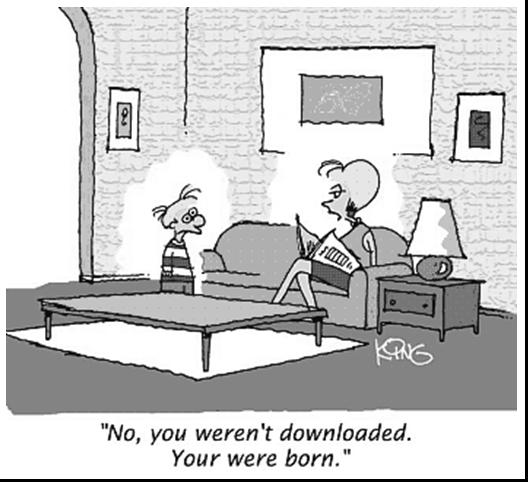
\includegraphics[width=.5\textwidth]{fig1.jpg}
\caption{A typical figure}
\label{fig:exampleFig1}
\end{figure}

\begin{figure}[ht]
\centering
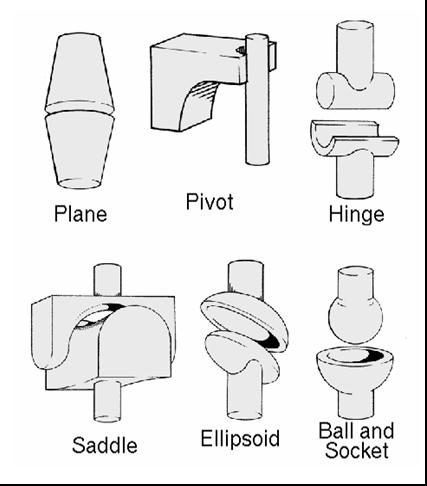
\includegraphics[width=.3\textwidth]{fig2.jpg}
\caption{This figure is an example of a figure caption taking more than one
  line and justified considering margins mentioned in Section~\ref{sec:figs}.}
\label{fig:exampleFig2}
\end{figure}

In tables, try to avoid the use of colored or shaded backgrounds, and avoid
thick, doubled, or unnecessary framing lines. When reporting empirical data,
do not use more decimal digits than warranted by their precision and
reproducibility. Table caption must be placed before the table (see Table 1)
and the font used must also be Helvetica, 10 point, boldface, with 6 points of
space before and after each caption.

\begin{table}[ht]
\centering
\caption{Variables to be considered on the evaluation of interaction
  techniques}
\label{tab:exTable1}
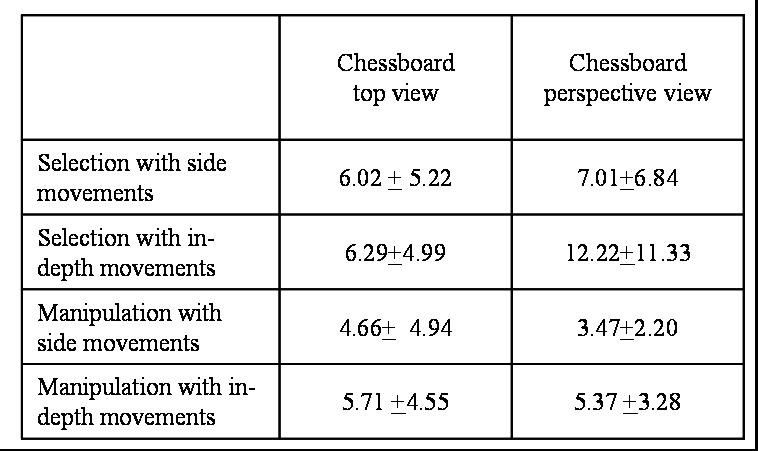
\includegraphics[width=.7\textwidth]{table.jpg}
\end{table}

\section{Images}

All images and illustrations should be in black-and-white, or gray tones,
excepting for the papers that will be electronically available (on CD-ROMs,
internet, etc.). The image resolution on paper should be about 600 dpi for
black-and-white images, and 150-300 dpi for grayscale images.  Do not include
images with excessive resolution, as they may take hours to print, without any
visible difference in the result. 

\section{References}

Bibliographic references must be unambiguous and uniform.  We recommend giving
the author names references in brackets, e.g. \cite{knuth:84},
\cite{boulic:91}, and \cite{smith:99}.

The references must be listed using 12 point font size, with 6 points of space
before each reference. The first line of each reference should not be
indented, while the subsequent should be indented by 0.5 cm.

\bibliographystyle{sbc}
\bibliography{sbc-template}

\end{document}
